\documentclass[../main.tex]{subfiles}
\begin{document}
\chapter{Analisi} 

\section{Analisi traffico di rete}

Nell'era digitale il traffico di rete è aumentato notevolmente e con esso gli attacchi di tipo informatico, per questo motivo è necessario trovare soluzioni per analizzare questo grande quantitativo di pacchetti che attraversano i dispositivi di rete delle aziende di grosse dimensioni. Nel mondo informatico di oggi è molto importante poter determinare rapidamente e con precisione l'origine e la portata di un potenziale attacco su una rete al fine di poterlo contrastare in modo efficace.
Per fare ciò viene costruito un \textit{audit trail}\footnote{Un audit trail è un file che contiene una registrazione cronologica di attività relative alla sicurezza per consentire la ricostruzione e l'esame di eventi \cite{auditTrail}.
} di informazioni collezionate dal traffico di rete usando una combinazione di network flow e packet capture.


\subsection{Packet Capture}
Per packet capture (PCAP) si intende la cattura di traffico internet che attraversa un dispositivo di rete; nel caso la cattura avvenga su un border router, è così possibile ispezionare tutto il traffico di rete generato da un'organizzazione. I software che si occupano di effettuare la cattura del traffico operano intercettando i singoli pacchetti, offrendo anche la possibilità di archiviarli su memoria persistente. Esempi di questi programmi sono la libreria \textbf{libpcap} per i sistemi operativi Unix, mentre sui sistemi Windows si fa utilizzo di \textbf{WinPcap} \cite{pcap}.

\subsection{Network Flow}
Un network flow è una sequenza di pacchetti inviati da una sorgente ad una destinazione che presentano degli attributi in comune \cite{trafficflow}, quali:
\begin{itemize}
				\item indirizzo IP sorgente
				\item indirizzo IP destinazione
				\item porta sorgente
				\item porta destinazione
				\item protocollo
\end{itemize}

Tutti i pacchetti che condividono gli stessi valori di questi attributi possono essere raggruppati in un unico flow. Risulta quindi evidente come le analisi basate sui network flow presentino numerosi vantaggi rispetto a quelle basate sui PCAP. Ad esempio, poichè i flow rappresentano un'aggregazione di pacchetti, è possibile diminuire drasticamente lo spazio richiesto per la memorizzazione. Di conseguenza, anche l'ispezione di tali dati risulterà più rapida e richiederà meno risorse computazionali. Va però sottolineato che i network flow non consentono di salvare il payload dei singoli pacchetti: questa caratteristica li rende da un lato meno dettagliati rispetto ai full packet capture; dall'altro, consente di effettuare l'analisi dei dati senza doversi preoccupare di questioni legate alla privacy degli utenti monitorati.

\subsubsection{NetFlow}
NetFlow~\cite{netflowDef} è un protocollo di analisi di rete introdotto da Cisco~\cite{netflowdef2} che offre la possibilità di raccogliere informazioni dettagliate sul traffico che attraversa un'interfaccia. I dispositivi di rete che supportano NetFlow possono raccogliere statistiche sul traffico ed esportarle come record verso un NetFlow collector, un server che esegue l'analisi del traffico.

Cisco definisce un flow come una sequenza unidirezionale di pacchetti che condividono tutti i seguenti 7 valori \cite{netflowDef}.

\begin{itemize}
				\item interfaccia di ingresso
				\item indirizzo IP sorgente
				\item indirizzo IP destinazione
				\item protocollo IP
				\item porta sorgente TCP o UDP, 0 per altri protocolli
				\item IP Type of Service
\end{itemize}

La figura ~\ref{fig:architetturaNetflow} descrive un esempio di architettura basata su NetFlow. 

\begin{figure}[H]
\centering
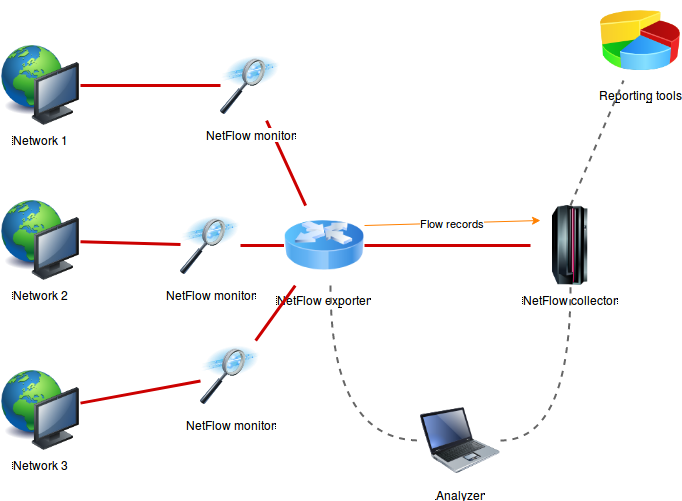
\includegraphics[scale=0.5]{netflowgraph.png}
\caption{Architettura NetFlow}
\label{fig:architetturaNetflow}
\end{figure}

\begin{verse}
\textbf{NetFlow monitor}
Un componente applicato a un'interfaccia che raccoglie informazioni sui flow. I NetFlow monitor sono costituiti da un record e una cache.
\end{verse}

\begin{verse}
\textbf{NetFlow exporter}
Aggrega i pacchetti in flows e ne esporta i record verso uno o più \textit{flow collectors}.
Quando dei pacchetti arrivano al NetFlow exporter, vengono ispezionati singolarmente per uno o più attributi che vengono utilizzati per determinare se il pachetto è univoco o è simile agli altri pacchetti. Se il pacchetto presenta attributi simili viene classificato nello stesso flow.
Dopo aver esaminato questi attributi, il NetFlow exporter li aggrega in record di flow e li salva in un database che può essere una cache NetFlow o un NetFlow collector. 

La figura ~\ref{fig:netflowExporter} rappresenta il funzionamento di un NetFlow exporter.

\begin{figure}[H]
\centering
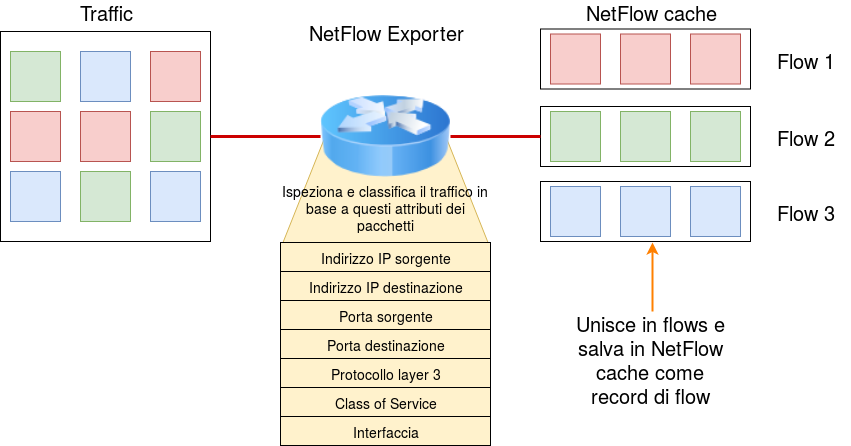
\includegraphics[scale=0.5]{netflowexporter.png}
\caption{NetFlow exporter}
\label{fig:netflowExporter}
\end{figure}

\end{verse}

\begin{verse}
\textbf{NetFlow collector}
Responsabile della ricezione, conservazione e pre-elaborazione dei dati di un flow ricevuti da un \textit{flow exporter}. Solitamente è un software separato in esecuzione su un server di rete. I record NetFlow vengono esportati in un NetFlow collector tramite protocollo UDP.
\end{verse}

\begin{verse}
\textbf{Analysis application} 
Analizza i dati dei flows ricevuti nel contesto del rilevamento delle intrusioni o del profilo di traffico. Un esempio di Analysis application possono essere degli IDPS.
L'immagine ~\ref{fig:solarwinds} rappresenta SolarWinds NetFlow Traffic Analyzer, un software per l'analisi dei flows \cite{solarwinds}.

\begin{figure}[H]
\centering
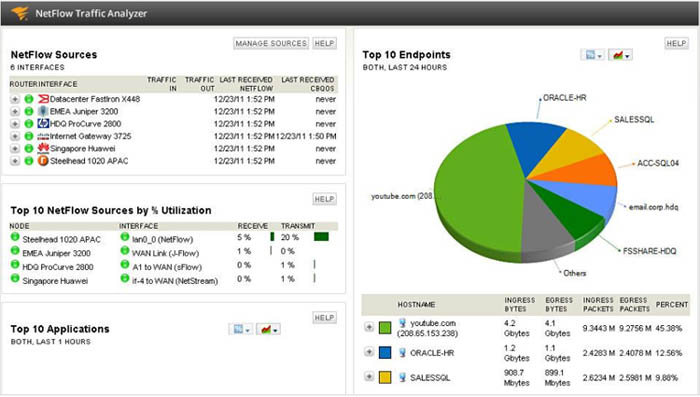
\includegraphics[scale=0.5]{netflowreport.jpg}
\caption{SolarWinds NetFlow Traffic Analyzer}
\label{fig:solarwinds}
\end{figure}
\end{verse}

\section{Strumenti di monitoraggio e analisi del traffico di rete}
In questa sezione verrano presentati i software per la cattura dei network flows che saranno oggetto di analisi di questa tesi: Argus e nProbe. Questi software sono Open Source e sono stati usati su una distribuzione GNU/Linux.

\subsection{Audit Record Generation and Utilization System}
Argus (Audit Record Generation and Utilization System) è stato la prima implementazione del monitoraggio dei flow, è un progetto open source e multipiattaforma \cite{Argus}.
Quest'ultima particolarità lo rende molto interessante poichè supportando molti sistemi operativi, tra i quali Windows, MacOSX, Linux, Solaris, FreeBSD, OpenBSD, IRIX e OpenWrt, può essere adoperato in quasi tutte le reti comprendendo la maggior parte degli host. La sua architettura è di tipo server/client. Il server recupera i pacchetti ricevuti da una o più interfacce di rete disponibili su una una macchina e Argus assembla poi questi pacchetti in dati binari che rappresentano dei flow. Lo scopo dei client è di quello di leggere i dati dei flow. 

Argus viene utilizzato da molte università e aziende~\cite{argusdef} per registrare dei flow che vengono utilizzati sia nell'analisi immediata dell'utilizzo della rete, sia nell'analisi storica.

I file di Argus sono compressi con algoritmi che offrono un rapporto di compressione fino 10.000:1. La compressione di questi file è molto importante perchè tendono ad essere molto grandi e possono raggiungere dimensioni difficili da gestire.


La tabella ~\ref{table:campiArgus} descrive i campi dei flow che argus salva su file. La prima colonna rappresenta il nome del campo del pacchetto di rete, la seconda colonna è una descrizione del campo.

\begin{table}[h]
				\centering
\begin{tabular}{|l|l|}
\hline
\textbf{campo} & \textbf{descrizione}                    \\ \hline
StartTime      & record start time                       \\ \hline
Dur            & record total duration                   \\ \hline
Proto          & transaction protocol                    \\ \hline
SrcAddr        & source IP address                       \\ \hline
Sport          & source port number                      \\ \hline
Dir            & direction of transaction                \\ \hline
DstAddr        & destination IP address                  \\ \hline
Dport          & destination port number                 \\ \hline
State          & transaction state                       \\ \hline
sTos           & source TOS byte value                   \\ \hline
dTos           & destination TOS byte value              \\ \hline
TotPkts        & total transaction packet count          \\ \hline
TotBytes       & total transaction bytes                 \\ \hline
SrcBytes       & src -\textgreater dst transaction bytes \\ \hline
srcUdata       & source user data buffer                 \\ \hline
dstUdata       & destination user data buffer            \\ \hline
Label          & metadata label                          \\ \hline
\end{tabular}\par
				\caption{Campi di Argus}
\label{table:campiArgus}
\end{table}

\subsection{nProbe}

Negli ambienti commerciali, NetFlow è probabilmente lo standard de facto per la gestione del traffico di rete. nProbe è un software in grado di reccogliere, analizzare ed esportare report sul traffico di rete utilizzando il formato standard Cisco NetFlow \cite{nProbe}. È disponibile per la maggior parte dei sistemi operativi sul mercato. 

La tabella ~\ref{table:campiNprobe} descrive i principali campi dei flow che nProbe è in grado di collezionare: nella colonna di sinistra si riporta il nome del campo, mentre viene fornita una breve descrizione corrispondente nella colonna di destra.

\begin{table}[H]
				\centering
\begin{tabular}{|l|l|}
\hline
\multicolumn{1}{|c|}{\textbf{campo}} & \multicolumn{1}{c|}{\textbf{descrizione}}     \\ \hline
IPV4\_SRC\_ADDR                      & IPv4 source address                           \\ \hline
IPV4\_DST\_ADDR                      & IPv4 destination address                      \\ \hline
IPV4\_NEXT\_HOP                      & IPv4 next hop address                         \\ \hline
INPUT\_SNMP                          & input interface SNMP idx                      \\ \hline
OUTPUT\_SNMP                         & output interface SNMP idx                     \\ \hline
IN\_PKTS                             & incoming flow packets (src -\textgreater dst) \\ \hline
IN\_BYTES                            & incoming flow bytes (src -\textgreater dst)   \\ \hline
FIRST\_SWITCHED                      & SysUptime (msec) of the first flow pkt        \\ \hline
LAST\_SWITCHED                       & SysUptime (msec) of the last flow pkt         \\ \hline
L4\_SRC\_PORT                        & IPv4 source port                              \\ \hline
L4\_DST\_PORT                        & IPv4 destination port                         \\ \hline
TCP\_FLAGS                           & cumulative of all flow TCP flags              \\ \hline
PROTOCOL                             & IP protocol byte                              \\ \hline
SRC\_TOS                             & Type of service byte                          \\ \hline
SRC\_AS                              & source BGP AS                                 \\ \hline
DST\_AS                              & destination BGP AS                            \\ \hline
IPV4\_SRC\_MASK                      & IPv4 source subnet mask                       \\ \hline
IPV4\_DST\_MASK                      & IPv4 dest subnet mask                         \\ \hline
L7\_PROTO                            & layer 7 protocol (numeric)                    \\ \hline
BIFLOW\_DIRECTION                    & 1=initiator, 2=reverseInitiator               \\ \hline
FLOW\_START\_SEC                     & seconds (epoch) of the first flow packet      \\ \hline
FLOW\_END\_SEC                       & seconds (epoch) of the last flow packet       \\ \hline
OUT\_PKTS                            & outgoing flow packets (dst -\textgreater src) \\ \hline
OUT\_BYTES                           & outgoing flow bytes (dst -\textgreater src)   \\ \hline
FLOW\_ID                             & serial flow identifier                        \\ \hline
FLOW\_ACTIVE\_TIMEOUT                & activity timeout of flow cache entries        \\ \hline
FLOW\_INACTIVE\_TIMEOUT              & inactivity timeout of flow cache entries      \\ \hline
IN\_SRC\_MAC                         & source MAC address                            \\ \hline
OUT\_DST\_MAC                        & destination MAC address                       \\ \hline
\end{tabular}\par
				\caption{Campi di nProbe}
\label{table:campiNprobe}
\end{table}

Rispetto ad Argus, nProbe è un software scalabile ed è stato progettato per restare al passo con le velocità multi-Gbit su hardware comune. Usando una CPU dual-core nProbe può essere usato per catturare pacchetti a 1 Gbit con perdita di pacchetti inferiore al 1\%. Inoltre nProbe permette una configurazione più dettagliata e personalizzabile, permette di scegliere molti campi per l'analisi dei network flow \cite{nProbe}.

Di contro, Argus è compatibile con un maggiore numero di sistemi: Mentre nProbe è disponibile solo per Unix, Windows o MacOs X, Argus funziona anche su FreeBSD, OpenBSD, NetBSD, AIX, HP-UX, VxWorks, IRIS e OpenWrt. inoltre è stato portato su molte piattaforme hardware accelerate come Bivio, Pluribus, Arista, Tilera \cite{Argus}. 

\section{Stratosphere Suite}
In questa tesi si è analizzata la Stratosphere Suite \cite{stratosphereSuite}, un insieme di software open source disponibile sia per sistemi operativi Windows che per le distribuzioni GNU/Linux. La Stratosphere Suite si compone di due parti distinte: Stratosphere IPS e Stratosphere Testing Framework.
Stratosphere IPS è un sistema di rilevazione e prevenzione delle intrusioni orientato all'analisi comportamentale basata sui network flow. L'obiettivo di Stratosphere IPS è quello di creare un Intrusion Prevention System in grado di rilevare e bloccare comportamenti malevoli all'interno di una rete. Si sottolinea che, per questa tesi, è stata utilizzata la versione di Stratosphere IPS per sistemi Linux (slips).
Stratosphere Testing Framework (stf) si occupa della generazione dei modelli comportamentali che saranno poi usati da Stratosphere IPS per effettuare le analisi del traffico e segnalare le possibili intrusioni.

\subsection{Stratosphere Linux IPS}
Slips si occupa della parte di rilevazione delle attività malevole impiegando algoritmi di machine learning che analizzano network flow. Questi algoritmi utilizzano i network flow in ingresso per elaborare dei modelli comportamentali in real-time di ciascun host monitorato: tali modelli comportamentali saranno quindi confrontati con dei modelli predefiniti che includono attività malevole. Nel caso slips riveli somiglianze significative tra i modelli "attuali" e quelli utilizzati per il confronto, genererà un allarme. 
Il processo di cattura dei network flow è effettuato attraverso Argus. L'idea di base è quella di leggere i flow da Argus e di inviarli a Slips. I modelli comportamentali da fornire a slips per effettuare il confronto vengono creati da Stratosphere Testing Framework.

La figura ~\ref{fig:architetturaStratosphere} descrive l'architettura della suite di Stratosphere. Su una rete interna o host singolo è presente un'istanza di Argus che cattura il traffico e crea dei network flow. La suite di Stratosphere protegge la rete interna tramite Slips che analizza il traffico catturato da Argus e stf che crea dei modelli comportamentali dai flows di Argus.

\begin{figure}[H]
\centering
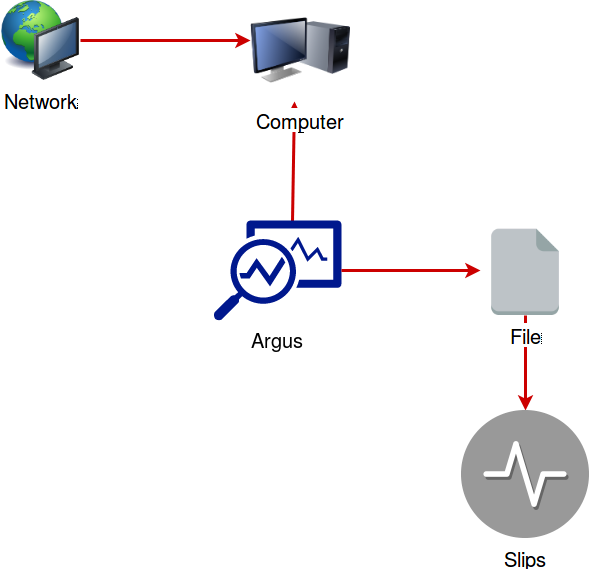
\includegraphics[scale=0.24]{archslips.png}
\caption{Architettura Stratosphere}
\label{fig:architetturaStratosphere}
\end{figure}



\subsection{Stratosphere Testing Framework}
Stf è un framework di ricerca sulla sicurezza della rete per analizzare i modelli comportamentali delle connessioni di rete. Il suo obiettivo è aiutare i ricercatori a trovare nuovi comportamenti malware, etichettare tali comportamenti, creare i loro modelli di traffico e verificare gli algoritmi di rilevamento. Una volta creati e verificati i migliori modelli comportamentali di malware, questi verranno utilizzati da slips per il rilevamento. Stratosphere Testing Framework usa algoritmi di machine learning sui modelli comportamentali.

Il nucleo di \textit{Stratosphere IPS} è composto dai modelli comportamentali di reti e algoritmi di rilevamento. I modelli comportamentali rappresentano ciò che una connessione specifica fa nella rete durante la sua vita. Per stf una connessione è un singolo flow, ovvero una sequenza di pacchetti che condividono dei valori. Il comportamento è costuito analizzando la sua periodicità, le dimensioni e la durata di ciascun flusso. Sulla base di queste caratteristiche a ciascun flusso viene assegnata una lettera e il gruppo di lettere caratterizza il comportamento della connessione.

Prendiamo come esempio una connessione generata da una botnet che ha il seguente modello comportamentale
\begin{lstlisting}[language=bash]
88*y*y*i*H*H*H*y*0yy*H*H*H*y*y*y*y*H*h*y*h*h*H*H*h*H*y*y*y*H*
\end{lstlisting}

In questo caso ci dice che i flussi sono altamente periodici (lettere \textit{h}, \textit{i}), con qualche periodicità persa vicino all'inizio (lettere \textit{y}). I flussi hanno anche una grande dimensione con una durata media. I simboli tra le lettere sono correlati al tempo trascorso tra i flussi. In questo caso il simbolo '\textit{*}' significa che il flusso è separato da meno di un'ora.
Con l'utilizzo di questo tipo di modelli siamo in grado di generare le caratteristiche comportamentali di un gran numero di azioni dannose. 

L'immagine ~\ref{fig:modelliComportamentali} mostra i criteri di assegnazione delle lettere per i modelli comportamentali.

\begin{figure}[H]
\centering
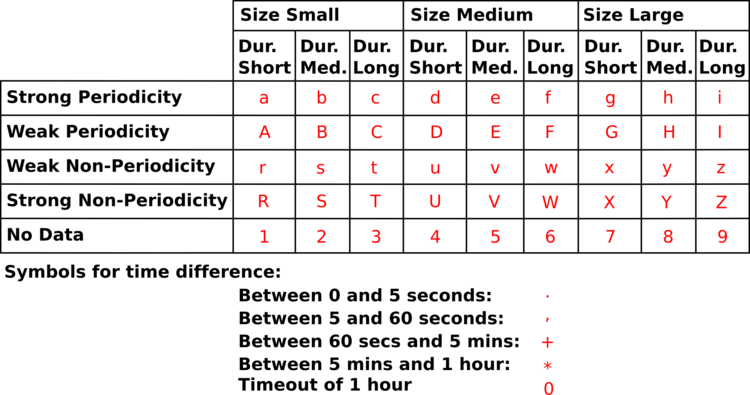
\includegraphics[scale=0.5]{modello-comportamentale.png}
				\caption{Tabella modelli comportamentali}
				\label{fig:modelliComportamentali}
\end{figure}

\section{Analisi del problema}
Questa tesi si occupa di risolvere un duplice problema: come installare ed utilizzare correttamente la suite di Stratosphere; come poter estendere la suite di Stratosphere utilizzando formati di netflow differenti da quelli prodotti da Argus.

\subsection{Deployment di Stratosphere IPS}
La suite di Stratosphere è attualmente pubblicata in alpha \cite{stratosphereSuite}. Un programma in alpha è un programma che è ancora nelle prime fasi di test e in genere include bug significativi e problemi di usabilità, pertanto se ne sconsiglia l'utilizzo in fasi di produzione \cite{alpha}.

Per l'installazione e l'utilizzo di questo software è stato necessario scaricare il codice sorgente da GitHub. Quando si esegue il programma scritto in Python \textit{slips.py} con il comando~\ref{lst:catslips}
\begin{lstlisting}[language=Bash, label={lst:catslips}, caption={comando per eseguire slips}]                                                                     
cat file.binetflow | ./slips.py -f models -d
\end{lstlisting}
L'output generato è vuoto e il programma non termina l'esecuzione. Si è provato con diversi file di netflow con gli stessi risultati, il programma sembra andare in loop senza mostrare alcun tipo di output. Si è quindi ispezionato il codice con tecniche di debug alla ricerca di una possibile soluzione per il corretto deployment del software.


\subsection{Problematiche dovute all'utilizzo di due diversi formati}
I file prodotti da nProbe e Argus, oltre ad avere formati diversi, hanno anche campi eterogenei. Stratosphere IPS si appoggia ad Argus per la cattura di file e di conseguenza può leggere file solo in formato binetflow. 
Se una azienda si appoggia a Cisco utilizzando nProbe non può quindi fare utilizzo di questo software, poichè non riesce a leggere file in formato differente.
I file prodotti da nProbe hanno una struttura gerarchica fissa ben definita: ci sono 4 livelli di subdir, in cui il primo livello indica l'anno, il secondo il mese, il terzo il giorno e il quarto l'ora. All'interno dell'ultima subdir, quella delle ore, ci sono 60 file uno per ogni minuto della giornata.
La immagine ~\ref{fig:folderStructure} descrive la struttura gerarchica dei file.

\begin{figure}[H]
\centering
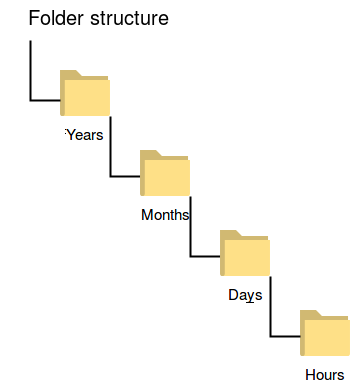
\includegraphics[scale=0.5]{folderstructure.png}
\caption{Folder Structure}
				\label{fig:folderStructure}
\end{figure}

Questa incompatibilità ha portato alla necessità di una conversione: i file prodotti da nProbe devono essere convertiti in file con formato usato da Argus. Questa conversione deve essere precisa (i.e., evitare al più possibile la perdita di informazioni) ed efficiente (i.e., essere eseguita in breve tempo in modo tale da poter utilizzare i flow convertiti per analisi in quasi real-time).





\end{document}
